\documentclass[beamer=true]{standalone}
\usepackage{../../preamblesnotes}

%Information to be included in the title page:
\title{第一課}
\author{運動學Kinematics}
\institute{全年班}
\date{}

\begin{document}
\frame{\titlepage}

\begin{frame}{長度和時間Length and Time}
    \begin{itemize}
        \item 運動學有兩個核心的物理量 - 長度和時間。\\There are two core physical quantities in kinematics, namely length and time.
        \item 長度的國際標準單位(S.I. 單位)是米(m)而時間的S.I.單位則是秒(s)。\\The units which belong to the international system (S.I. units) of lengths and time durations are meters (m) and seconds (s) respectively.
    \end{itemize}
\end{frame}
\begin{frame}{長度和時間Length and Time}
    當我們要表述極大或極小的物理量時,我們可在單位前方加上單位接頭,如下表所示。\\We can use a prefix to represent an enormous or tiny quantity as shown below.
    \begin{figure}[h!]
        \centering
        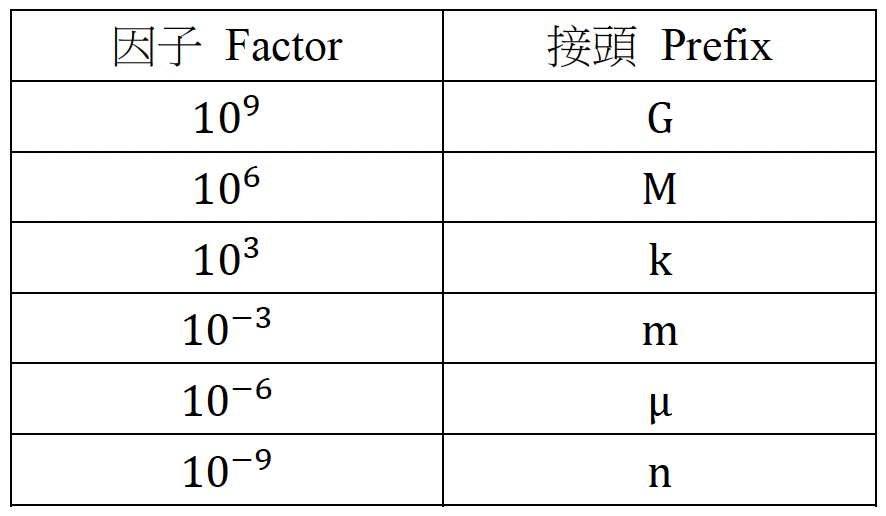
\includegraphics[width=.5\textwidth]{../../assets/3d0d2672.png}
    \end{figure}
\end{frame}

\begin{frame}{純量scalars}
    \begin{itemize}
        \item 標量/純量是一種物理量,只具備\textbf{量值}(大小)而沒有方向。\\A scalar is a physical quantity that only possesses \textbf{magnitude} (size).
              \begin{itemize}
                  \item 純量的例子:質量、能量、長度、體積、時間等等。\\s of scalar: mass, energy, length, volume, time, etc.
              \end{itemize}
        \item 純量在大部分情況下都是正數。但是也可以是負數。(例如:勢能,作功)\\A scalar is positive in most cases, but it can be negative. (e.g. potential energy, work done)
    \end{itemize}
\end{frame}

\begin{frame}{向量vectors}
    \begin{itemize}
        \item 向量/矢量同時具備\textbf{量值}和\textbf{方向}。\\A vector is a physical quantity that possesses both \textbf{magnitude} (size) and \textbf{direction}.
              \begin{itemize}
                  \item 在一維問題中,使用正負號$(+ \textrm{ 或 }\, -)$來表示方向。\\In a one-dimensional problem, a sign $(+ \textrm{ or } -)$ is used to represent direction.
                  \item 在二維問題中,向量能用箭號來表示\textbf{方向},箭號的\textbf{長度}表示向量的\textbf{量值}。\\In a two-dimensional problem, a vector can be represented by an arrow to indicate its \textbf{direction} and the \textbf{length} represents its \textbf{magnitude}.
              \end{itemize}
        \item 向量的例子:位移、速度、加速度、力、動量等等。\\s of vector: displacement, velocity, acceleration, force and momentum etc.
    \end{itemize}

\end{frame}


\begin{frame}{向量vectors}

    \begin{itemize}
        \item 向量的量值必定是\textbf{正}數。\\The magnitude of a vector must be a \textbf{positive} value.
        \item 例:比較A、B、C的速度的量值。\\: compare the magnitude of A, B, and C.\par A:\qty{-20}{m.s^{-1}}、B:\qty{10}{m.s^{-1}}、C:\qty{-30}{m.s^{-1}}\par 答案Answer: C>B>A
    \end{itemize}

\end{frame}

\begin{frame}{向量vectors}
    \begin{itemize}
        \item 例如圖中的向量的量值是$2\sqrt{2}$cm,方向是東北方。 \\For , the magnitude of the vector on the right is $2\sqrt{2}$cm and the direction of the vector is N.E.
        \item 因為右方的向量從A點指向B點,因此可記為$\vec{AB}$。 \\Since the vector on the right points from point A to point B, so it can be denoted as $\vec{AB}$.
        \item
              向量可平移而不受改變。\\Vectors can be translated without changing.
    \end{itemize}
    \begin{figure}[h!]
        \centering
    \end{figure}
\end{frame}
\begin{frame}{向量的加法︰平行四邊形法Addition of vector: Parallelogram method}
    \begin{figure}[h!]
        \centering
        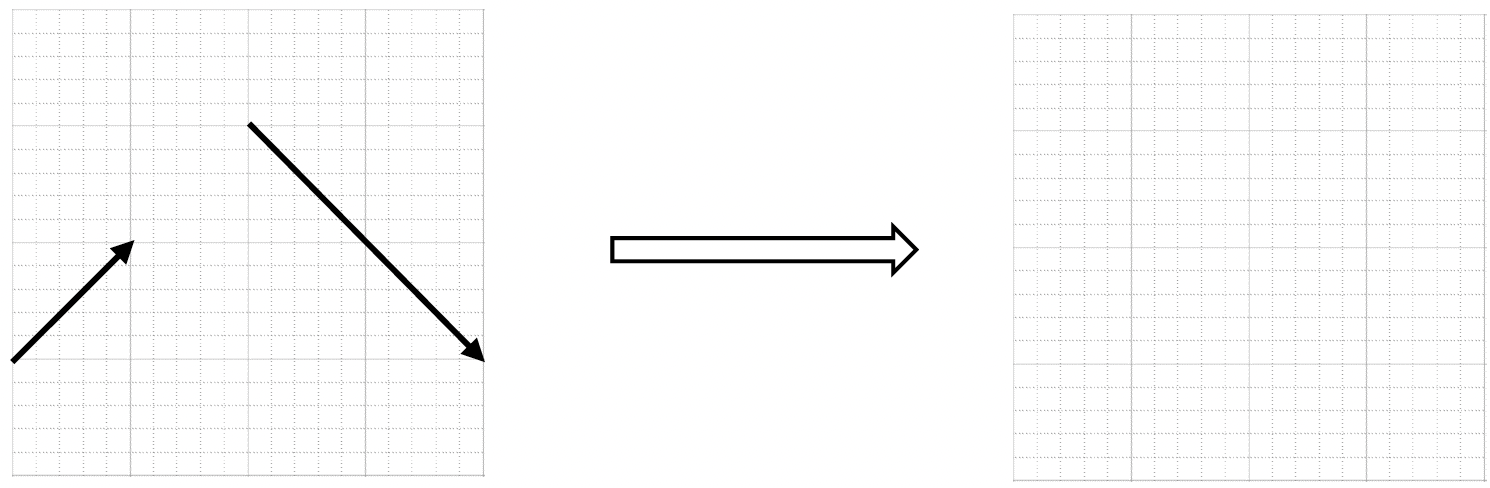
\includegraphics[width=.9\textwidth]{../../assets/3cc60b5d.png}
    \end{figure}
    \begin{figure}[h!]
        \centering
        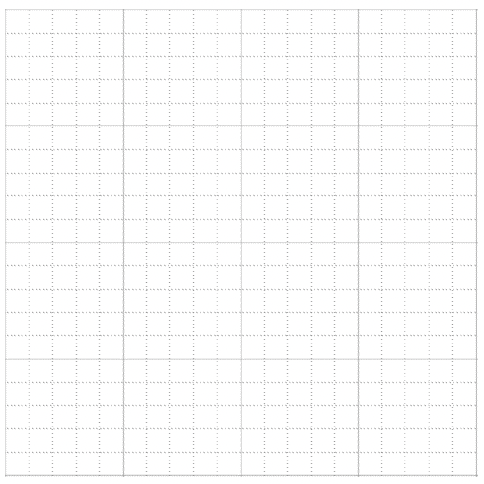
\includegraphics[width=.3\textwidth]{../../assets/45d03651.png}
    \end{figure}
\end{frame}
\begin{frame}{向量的加法︰首尾相接法Addition of vector: Tip-to-tail method}
    \begin{figure}[h!]
        \centering
        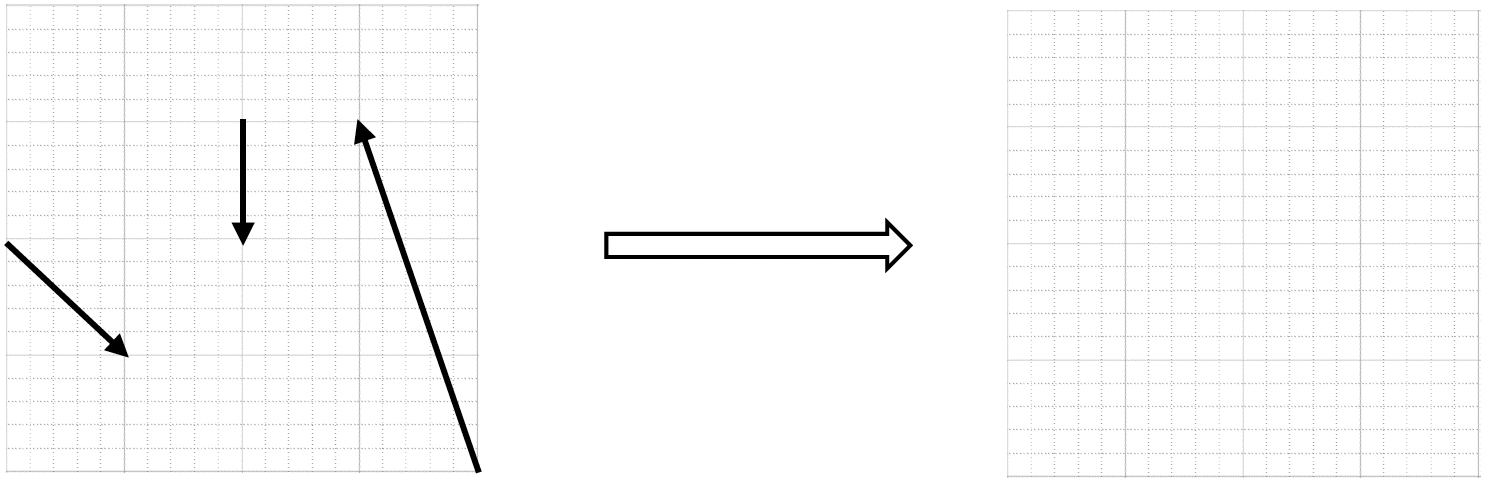
\includegraphics[width=.9\textwidth]{../../assets/b696d9b0.png}
    \end{figure}
    \begin{figure}[h!]
        \centering
        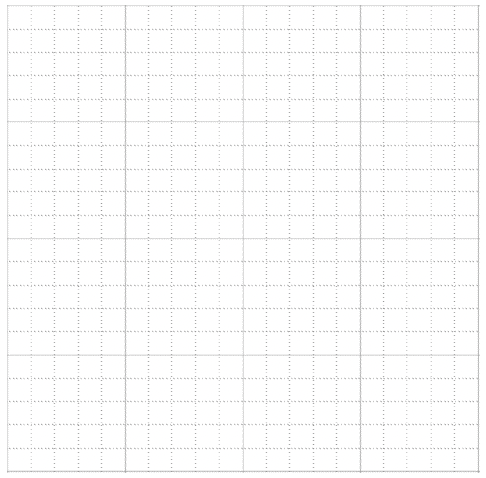
\includegraphics[width=.3\textwidth]{../../assets/af91e6db.png}
    \end{figure}
\end{frame}
\begin{frame}{向量的加法︰平行四邊形法Addition of vector: Parallelogram method}
    \begin{figure}[h!]
        \centering
        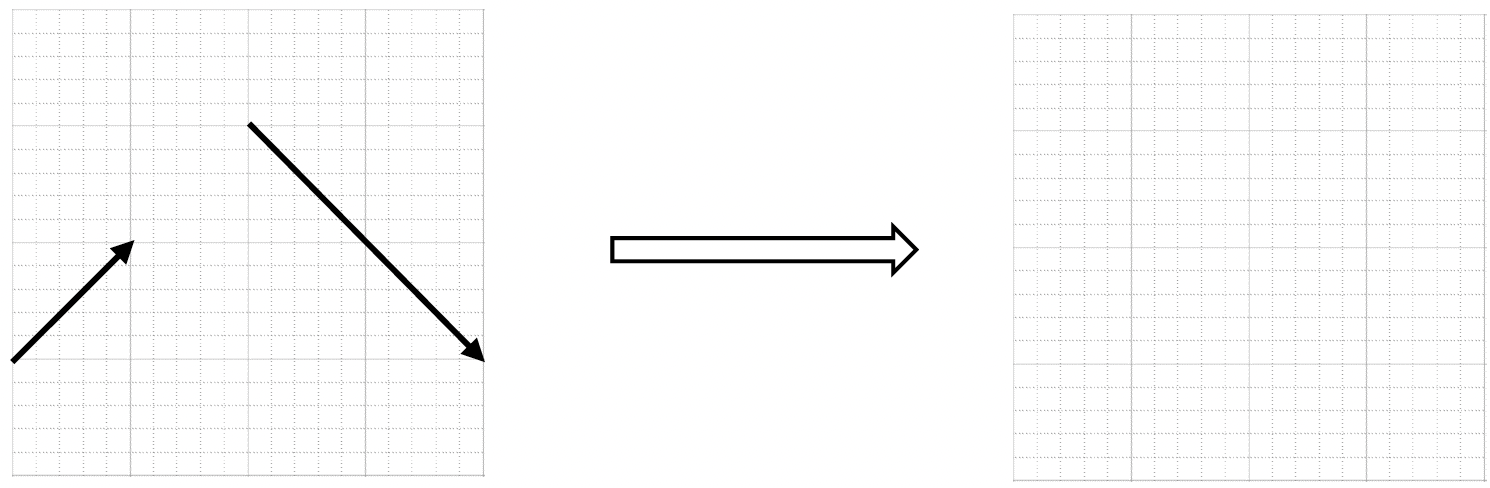
\includegraphics[width=.9\textwidth]{../../assets/3cc60b5d.png}
    \end{figure}
    \begin{figure}[h!]
        \centering
        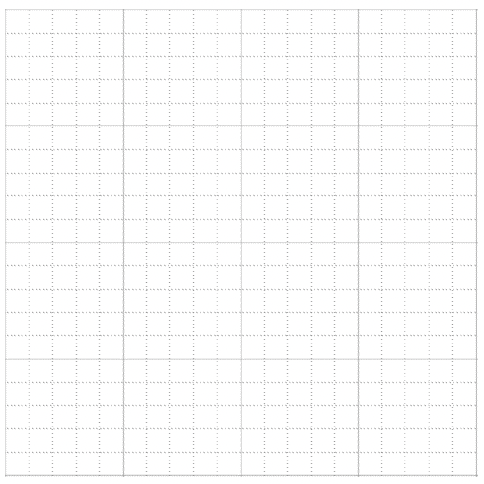
\includegraphics[width=.3\textwidth]{../../assets/45d03651.png}
    \end{figure}
\end{frame}

\begin{frame}{例題}
    求以下各圖中所有向量的總和的量值。\\Find the magnitudes of the sum of all vectors in each diagram.
    \begin{figure}[h!]
        \centering
        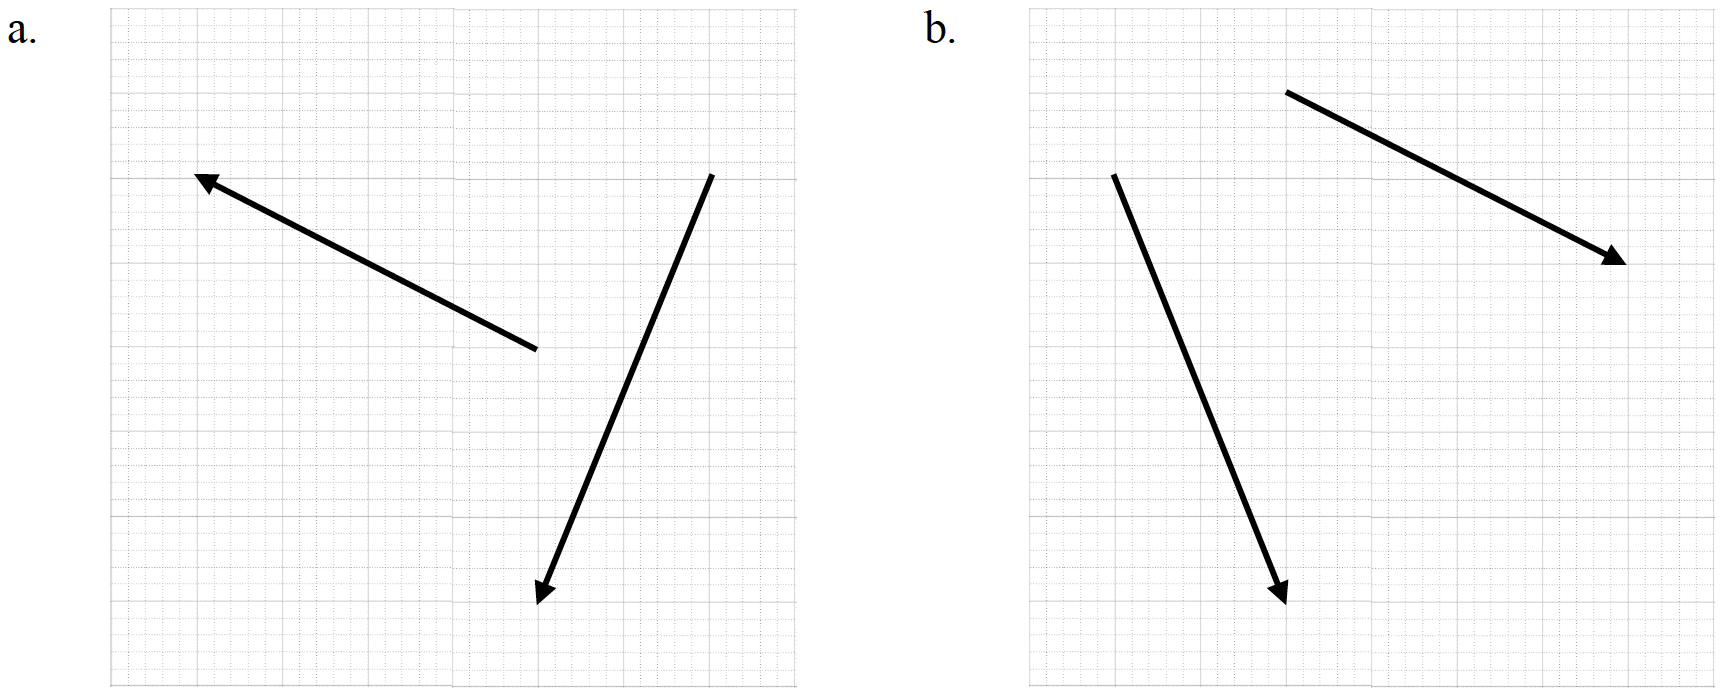
\includegraphics[width=\textwidth]{../../assets/b3abd67b.png}
    \end{figure}
\end{frame}
\begin{frame}{例題}
    求以下各圖中所有向量的總和的量值。\\Find the magnitudes of the sum of all vectors in each diagram.
    \begin{figure}[h!]
        \centering
        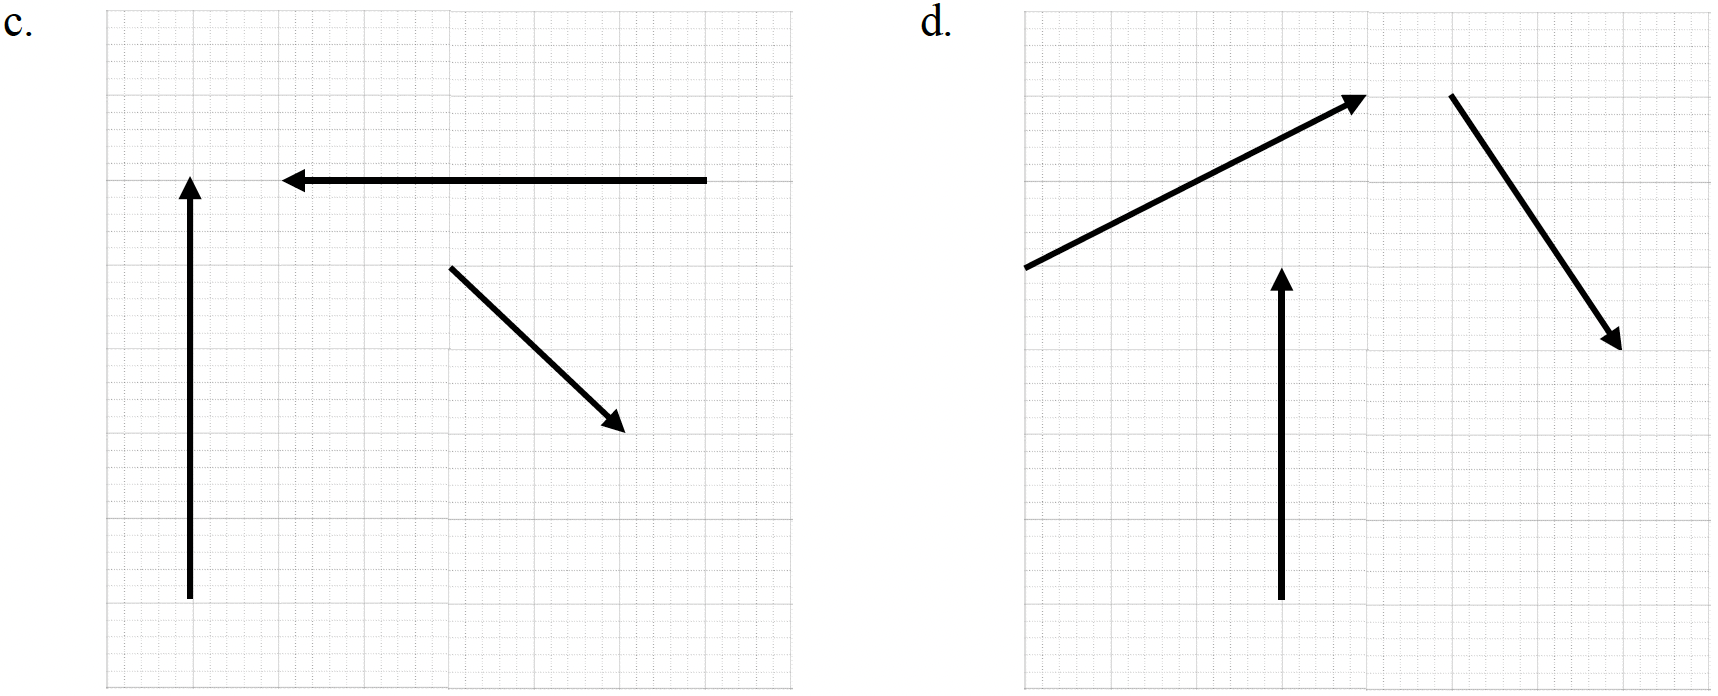
\includegraphics[width=\textwidth]{../../assets/2d454bed.png}
    \end{figure}
\end{frame}
\begin{frame}{例題}
    已知以下的向量加法算式成立,在空白的圖中畫出缺少的向量。 \\It is given that the addition expressions of the vectors hold true, draw the missing vectors in the blank diagrams.
    \begin{figure}[h!]
        \centering
        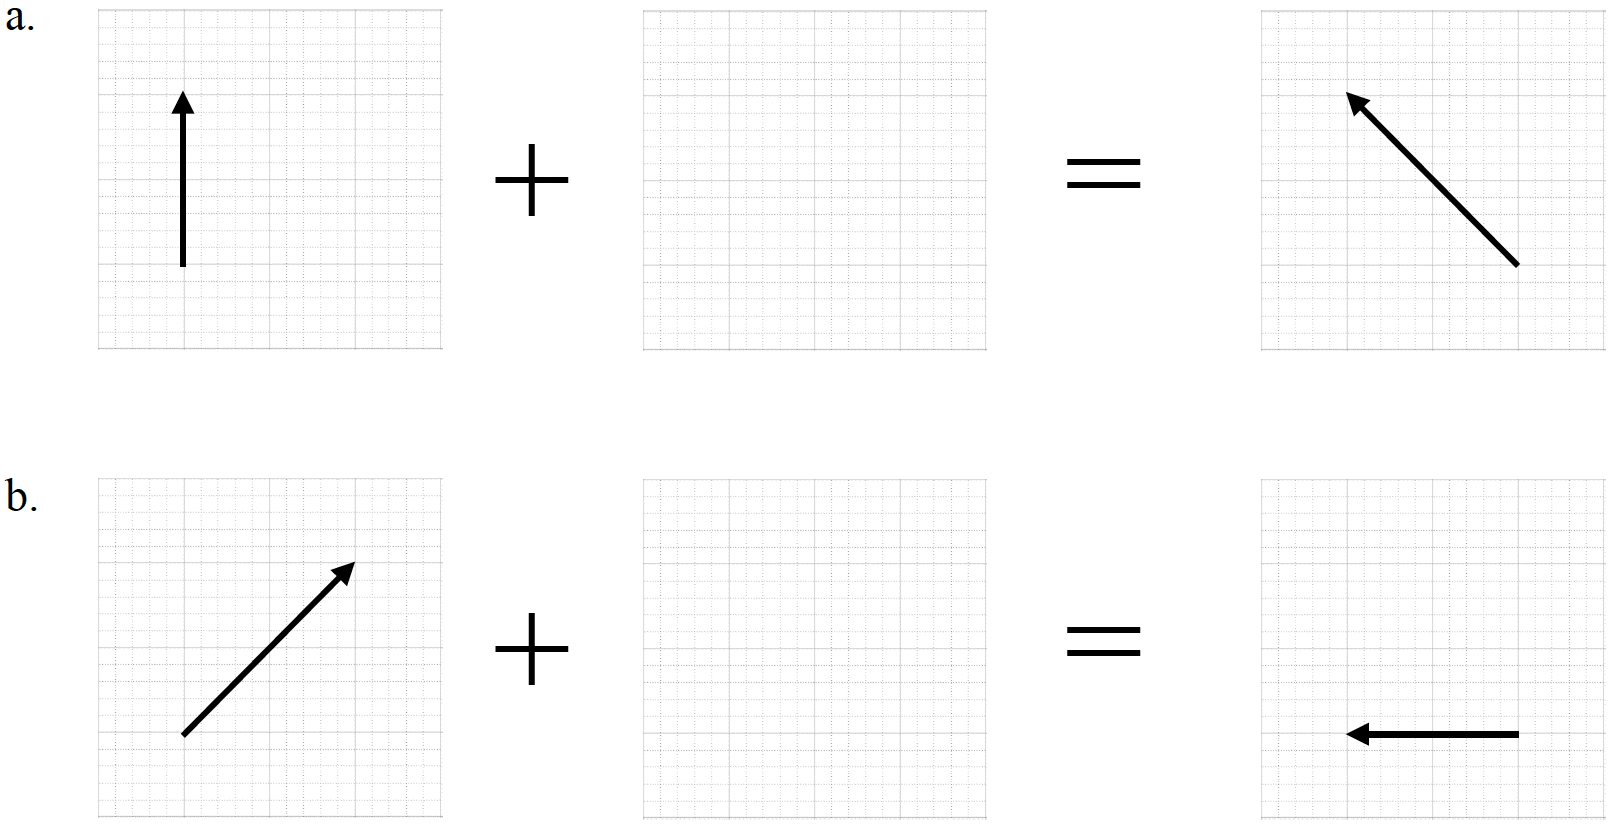
\includegraphics[width=\textwidth]{../../assets/02f3ce52.png}
    \end{figure}
\end{frame}
\begin{frame}{例題}
    已知以下的向量加法算式成立,在空白的圖中畫出缺少的向量。 \\It is given that the addition expressions of the vectors hold true, draw the missing vectors in the blank diagrams.
    \begin{figure}[h!]
        \centering
        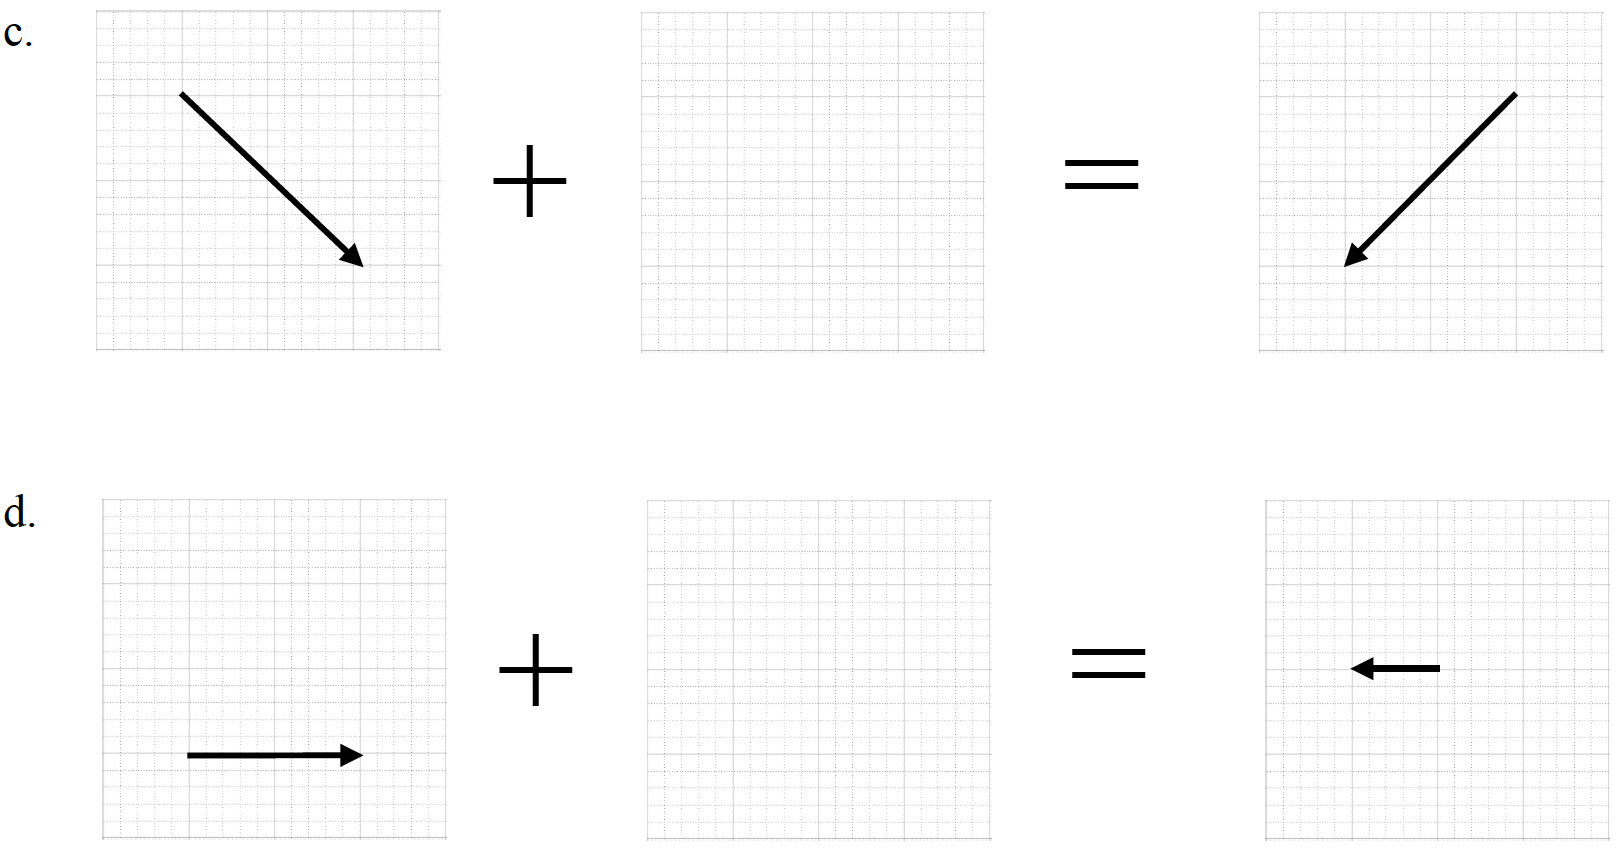
\includegraphics[width=\textwidth]{../../assets/9088f28e.png}
    \end{figure}
\end{frame}
\begin{frame}[t]{例題}
    已知以下的向量加法算式成立,在空白的圖中畫出缺少的向量。 \\It is given that the addition expressions of the vectors hold true, draw the missing vectors in the blank diagrams.\bigskip
    \begin{figure}[h!]
        \centering
        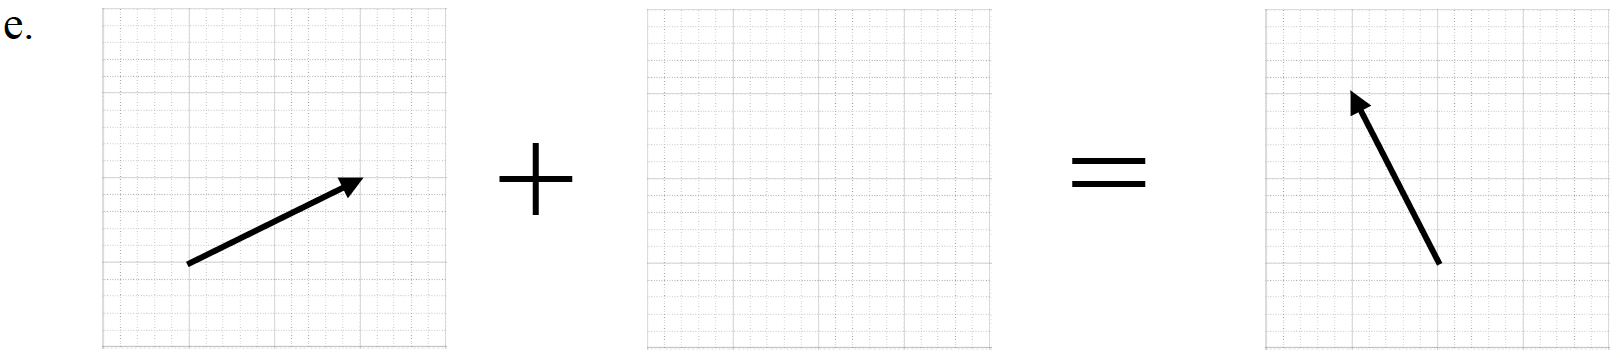
\includegraphics[width=\textwidth]{../../assets/6767fde4.png}
    \end{figure}
\end{frame}

\begin{frame}{位移和距離 Displacement and distance}
    \begin{itemize}
        \item 當一個運動的物件從P點移動到Q點,我們可以討論這物件的位移和距離。 \\When a moving object moves from point P to Q, we can talk about its displacement.
        \item 位移是向量,它只取決運動的\textbf{起點}和\textbf{終點}。\\A displacement is a vector, it only depends on the \textbf{starting} and \textbf{finishing point} of the motion.
        \item 量值是P點和Q點之間的直線距離,而方向則從P點指向Q點。\\The magnitude of a displacement equals the straight distance between the starting point and ending point of the motion.
        \item 因此,位移與運動的軌跡無關。 \\Therefore, displacements are independent to motion trajectories.
        \item 距離是純量,它表達的是從P點到Q點運動的\textbf{完整軌跡}。
              \\A distance is a scalar, it represents the \textbf{complete trajectory} from P to Q.
    \end{itemize}
\end{frame}


\begin{frame}[t]{例題}
    對以下各路程,求總距離和合位移的量值。 \\For each of the following journeys, find the total distance and the magnitudes of the resultant displacements.
    \begin{itemize}
        \item [(a)]先向北前進 20 m,再向東前進 25 m。 \\Proceed 20 m due North, and then proceed 25 m due East.
    \end{itemize}
\end{frame}
\begin{frame}[t]{例題}
    對以下各路程,求總距離和合位移的量值。 \\For each of the following journeys, find the total distance and the magnitudes of the resultant displacements.
    \begin{itemize}
        \item [(b)] 向右走 10 m,其後向前走 4 m,最後向左走 7 m。 \\Walk 10 m to the right, and then 4 m forward, finally 7 m to the left.
    \end{itemize}
\end{frame}
\begin{frame}[t]{例題}
    對以下各路程,求總距離和合位移的量值。 \\For each of the following journeys, find the total distance and the magnitudes of the resultant displacements.
    \begin{itemize}
        \item [(c)] 先向 N \qty{60}{^\circ} E 前進 2.4 km,其後再西前進 6 km。 \\Proceed 2.4 km alone N \qty{60}{^\circ} E, and then move 6 km due West.
    \end{itemize}
\end{frame}
\begin{frame}[t]{例題}
    對以下各路程,求總距離和合位移的量值。 \\For each of the following journeys, find the total distance and the magnitudes of the resultant displacements.
    \begin{itemize}
        \item [(d)] 向北、向東、向南、向西依次各走 20 m。 \\Go North, East, South and West respectively, each for 20 m.
    \end{itemize}
\end{frame}

\begin{frame}{速率 Speed}
    \begin{itemize}
        \item 速率是\textbf{純量},它不顯示物體移動的方向,只表示物體移動的快慢。 \\Speeds are \textbf{scalar}, speed does not show the directions of the moving objects but only how fast the object moves.
        \item 速率的SI單位是米每秒,可寫作 \unit{m.s^{-1}}。 \\The S.I. unit of speed is meter per second, which can be written as \unit{m.s^{-1}}.
        \item 另一個常見的單位是千米每小時(\unit{km.h^{-1}})。 Another common unit of speed is kilometers per hour (\unit{km.h^{-1}}).
        \item []$1\unit{km.h^{-1}}=\dfrac{5}{18}\unit{m.s^{-1}}$

    \end{itemize}

\end{frame}
\begin{frame}{速率 Speed}
    \begin{itemize}
        \item \textbf{平均速率}是物件在整個旅程中移動快慢的概觀,計算方法如下︰ \\\textbf{Average speed} is the overview of how fast the object moves in the whole journey, it can be calculated as follows:
              \begin{itemize}
                  \item[] $\textrm{平均速率 Average speed}=\dfrac{\textrm{移動的距離 Moving distance}}{\textrm{所需時間 Time needed}}$
              \end{itemize}
        \item 物體在某一瞬間的速率稱為\textbf{瞬時速率},它等於極短時距內的平均速率。\\ The \textbf{instantaneous speed} of an object equals the average speed in a very short time interval, it measures the speed of the object in a very brief moment.
    \end{itemize}

\end{frame}
\begin{frame}{速度 Velocity}
    \begin{itemize}
        \item 速度是向量,它顯示物體移動的快慢和方向,定義如下︰ \\Velocities are vectors which show the directions and how fast the objects move and are defined as follow:
        \item 速度 Velocity=每單位時間內物體的位移 Displacement of an object per unit time
        \item 速度的SI單位是米每秒,可寫作 \unit{m.s^{-1}}。 \\The S.I. unit of velocities is meter per second, which can be written as \unit{m.s^{-1}}.
        \item 平均速度計算方法與平均速率類似,計算方法如下︰ \\The way of calculating average velocities is similar to that of average speeds as shown:
        \item []$\textrm{平均速度 Average velocity}=\dfrac{\textrm{總位移 Total displacement}}{\textrm{所需時間 Time needed}}$
    \end{itemize}

\end{frame}

\begin{frame}{速度 Velocity}
    \begin{itemize}
        \item 物體在某一瞬間的速度稱為\textbf{瞬時速度},它等於極短時間內的平均速度。\\The \textbf{instantaneous velocity} of an object equals the average velocity in a very short time interval, it measures the velocity of the object in a certain instant.
        \item 任何物體的瞬時速度量值等於瞬時速率。\\The magnitude of the instantaneous velocity of any object equals to the instantaneous speed.

    \end{itemize}

\end{frame}
\begin{frame}{速度 Velocity}
    \begin{itemize}

        \item 物體以恆速率移動時,速度不一定恆定不變。 \\When an object is moving at constant speed, its velocity does not necessarily change.
        \item 若物體以恆速度移動,那麼它所做的就是\textbf{勻速運動}。 \\If an object is moving at a constant velocity, then the object is said to be performing \textbf{uniform motion}.
    \end{itemize}

\end{frame}

\begin{frame}[t]{例題}
    求以下過程的平均速度量值及平均速率。 \\Find the magnitudes of average velocities and average speeds for each of the following journeys.
    \begin{itemize}
        \item [(a)]在5 s內向東走2 m,其後立即在3 s內向北走5 m。 \\Walk 2 m due East in 5 s, and then immediately walk 5 m due North for 3 s.
    \end{itemize}
\end{frame}
\begin{frame}[t]{例題}
    求以下過程的平均速度量值及平均速率。 \\Find the magnitudes of average velocities and average speeds for each of the following journeys.
    \begin{itemize}
        \item [(b)]先以 \qty{40}{km.h^{-1}} 的速率向北行駛,其後馬上以 \qty{60}{km.h^{-1}} 原路折返至起點。 \\Drive \qty{40}{km.h^{-1}} due North, and then return to the starting point along the same path at \qty{60}{km.h^{-1}}.
    \end{itemize}
\end{frame}
\begin{frame}[t]{例題}
    求以下過程的平均速度量值及平均速率。 \\Find the magnitudes of average velocities and average speeds for each of the following journeys.
    \begin{itemize}
        \item [(c)]向西走20 m後再北走30 m,然後升電梯向上升50 m。合共需時 80 s。 \\Walking 20 m due west and the 30 m due north, and then move upward by 50 m in an elevator. 80 s is elapsed in total.
    \end{itemize}
\end{frame}
\begin{frame}[t]{例題}
    一輛車以 40 s 通過一條半圓形的路段。在這段期間,車速計始終顯示如下。\\ A car passes through a semi-circular road in 40 s. The speedometer reads as follow throughout the whole time interval.
    \begin{figure}[h!]
        \centering
        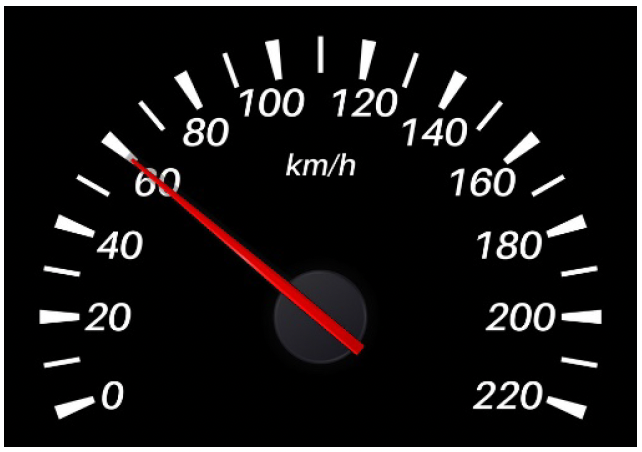
\includegraphics[width=.35\textwidth]{../../assets/fca35903.png}
    \end{figure}
    \begin{itemize}
        \item [(a)]寫出車速計顯示的是什麼物理量。 \\Write down the what the physical quantity is shown by the speedometer.
    \end{itemize}
\end{frame}
\begin{frame}[t]{例題}

    \begin{itemize}
        \item [(b)]Calculate the magnitude of the average velocity during the 40 s. \\計算在40 s內的平均速度量值。
    \end{itemize}
\end{frame}
\begin{frame}[t]{例題}

    \begin{itemize}
        \item [(c)]指出以下命題是否\textbf{可能}為真。\\State if each the following statements \textbf{can be} true or not.
              \begin{itemize}
                  \item [(i)]該車在該40 s內某些時刻超過 \qty{70}{km.h^{-1}}。\\The vehicle exceeds \qty{70}{km.h^{-1}} at some moment in the 40 s interval.
              \end{itemize}
    \end{itemize}
\end{frame}
\begin{frame}[t]{例題}

    \begin{itemize}
        \item [(c)]指出以下命題是否\textbf{可能}為真。\\State if each the following statements \textbf{can be} true or not.
              \begin{itemize}
                  \item [(ii)]在該40 s內,車的速度始終不變。\\The velocity of the car stays unchanged thoughout the 40 s.
              \end{itemize}
    \end{itemize}
\end{frame}
\begin{frame}{加速度 Accelerations}
    \begin{itemize}
        \item 加速度定義為速度的變化率︰ \\The rate of change of the velocity of an object is known as acceleration:
        \item 加速度 Acceleration=單位時間內物體的速度變化 Velocity change of the object in unit time
        \item 加速度是向量,它的S.I.單位是米每平方秒,即 \unit{m.s^{-2}}。 Accelerations are vectors, the unit in S.I. unit meters per second squared (\unit{m.s^{-2}}).
    \end{itemize}
\end{frame}
\begin{frame}{加速度 Accelerations}
    \begin{itemize}
        \item 當物體的速度在一段時間內出現變化,它的平均加速度可利用下式求得︰\\When the velocity of on object changes in an interval, its average acceleration can be calculated as follow:
        \item $\textrm{平均加速度 Average acceleration}=\dfrac{\textrm{速度的總變化 Overall change in velocity}}{\textrm{所需時間 Time elapsed}}$
        \item 物體的瞬時加速度是極短時段內的平均加速度。 \\The instantaneous acceleration of an object is the average acceleration in a very brief time interval.
    \end{itemize}
\end{frame}
\begin{frame}{加速度 Accelerations}
    \begin{itemize}
        \item 當物體受重力落下,且其間不受其他因素影響,這個落下運動稱為自由下落。自由下落的勻加速度稱為重力加速度,符號為 $\mathit{g}$。 \\When an object falls under the influence of gravity but not other factors, the falling motion is known as free-falling. The acceleration of the free-falling object is known as gravitational acceleration, and is denoted as $\mathit{g}$.
        \item 在地球表面,$\mathit{g}$ = \qty{9.81}{m.s^{-2}}。 \\On earth surface, $\mathit{g}$ = \qty{9.81}{m.s^{-2}}.
    \end{itemize}
\end{frame}
\begin{frame}[t]{例題}
    一個粒子初時以 \vel{1.6} 的速率沿直線運動。4 s 後,這粒子的速率是 \vel{4.8}。求這粒子在 4 s 內所有可能的平均加速度量值。 \\A particle is moving along a straight line at the speed \vel{1.6} initially. 4 s later, the speed of the particle becomes \vel{4.8}. Find the magnitudes of all of the possible average accelerations.
\end{frame}
\begin{frame}[t]{例題}
    一隻螞蟻站在某時鐘的秒針末端。已知秒針長度是10 cm。計算這螞蟻在 30 s 內的平均加速度量值。
\end{frame}
\begin{frame}[t]{例題}
    一輛車先以 \kmh{40} 的速率向南行駛,其後以 \kmh{50} 的速率向西行駛。車花費了 20 s 拐彎。
    \begin{itemize}
        \item [(a)]求車的速度改變量值及方向。
    \end{itemize}
\end{frame}
\begin{frame}[t]{例題}
    一輛車先以 \kmh{40} 的速率向南行駛,其後以 \kmh{50} 的速率向西行駛。車花費了 20 s 拐彎。
    \begin{itemize}
        \item [(b)]求車拐彎期間的平均加速度量值。
    \end{itemize}
\end{frame}
\begin{frame}[t]{例題}
    一個物件以初速度u垂直向上拋。在2 s後及4 s後,這物件的速率相同。求u的量值。取 $\mathit{g}=$\acc{9.81}。
\end{frame}

\begin{frame}{位移–時間關係線圖 Displacement–time graph}
    \begin{itemize}
        \item 位移–時間關係線圖簡稱 s-t 線圖,顯示物體在不同時刻相對於參考點的位移。線圖的橫軸代表時間,縱軸則代表位移。
        \item 線圖的\textbf{斜率}等於物件的\textbf{瞬時速度}。
    \end{itemize}
\end{frame}
\begin{frame}{速度–時間關係線圖 Velocity–time graph}
    \begin{itemize}
        \item 速度–時間關係線圖簡稱 v-t 線圖,顯示物體在不同時刻的速度。線圖的橫軸代表時間,縱軸則代表速度。
        \item 線圖的\textbf{鈄率}等於物件的\textbf{瞬時加速度}。
        \item 線圖與橫軸之間的\textbf{面積} 等於物件的\textbf{位移}。
    \end{itemize}
\end{frame}

\begin{frame}{加速度–時間關係線圖}
    \begin{itemize}
        \item 加速度–時間關係線圖簡稱 a-t 線圖,顯示物體在不同時刻的加速度。線圖的橫軸代表時間,縱軸則代表加速度。
        \item 線圖與橫軸之間的 \textbf{面積}等於物件的\textbf{速度改變}。
    \end{itemize}
\end{frame}

\begin{frame}[t]{例題}
    一個粒子的位移 s 如圖隨時間 t 變化。
    \begin{figure}[h!]
        \centering
        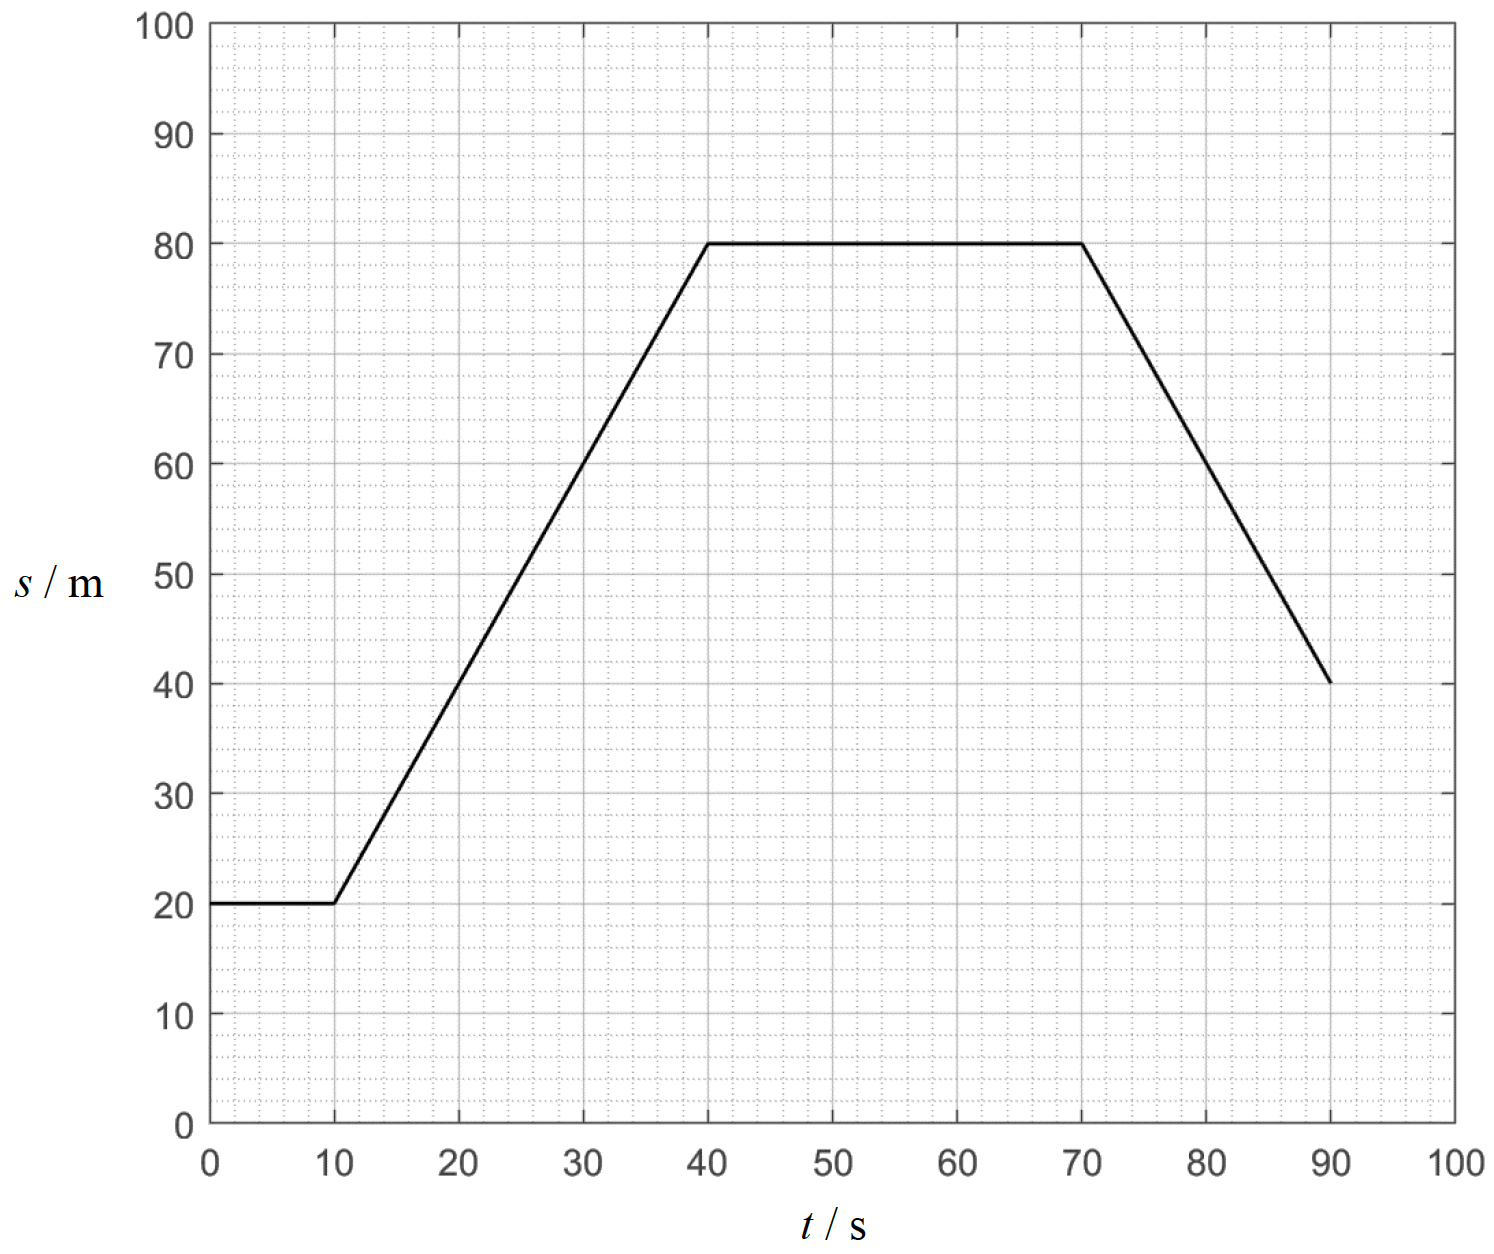
\includegraphics[width=0.61\textwidth]{../../assets/07c55dd0.png}
    \end{figure}
\end{frame}
\begin{frame}[t]{例題}
    求以下各項。
    \begin{itemize}
        \item [(a)]在 t = 20 s 時的瞬時速度。
    \end{itemize}
\end{frame}
\begin{frame}[t]{例題}
    求以下各項。
    \begin{itemize}
        \item [(b)]在 $t = 10-50 $ \unit{s} 期間的平均速度。
    \end{itemize}
\end{frame}
\begin{frame}[t]{例題}
    求以下各項。
    \begin{itemize}
        \item [(c)]在 t = 5 s 時的瞬時速度。
    \end{itemize}
\end{frame}
\begin{frame}[t]{例題}
    求以下各項。
    \begin{itemize}
        \item [(d)]在 t = 5 – 20 s 期間的平均加速度量值。
    \end{itemize}
\end{frame}
\begin{frame}[t]{例題}
    以下是一輛車的速度–時間線圖。
    \begin{figure}[h!]
        \centering
        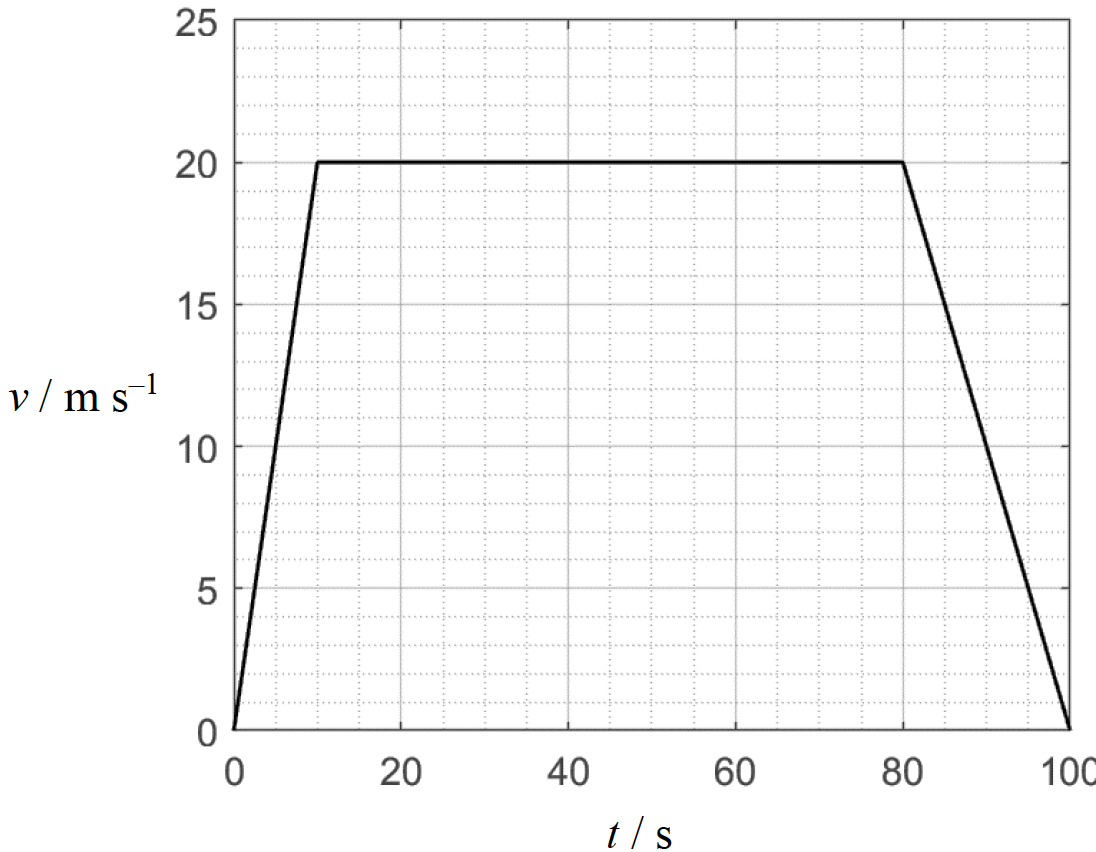
\includegraphics[width=0.7\textwidth]{../../assets/595e8206.png}
    \end{figure}
\end{frame}
\begin{frame}[t]{例題}
    \begin{itemize}
        \item [(a)]描述車的運動。
    \end{itemize}
\end{frame}
\begin{frame}[t]{例題}
    \begin{itemize}
        \item [(b)]求車在 t = 95 s 時的加速度量值。
    \end{itemize}
\end{frame}
\begin{frame}[t]{例題}
    \begin{itemize}
        \item [(c)]求車在這 100 s 中前進的距離。
    \end{itemize}
\end{frame}
\begin{frame}{例題}
    以下是一輛車的速度–時間線圖。
    \begin{figure}[h!]
        \centering
        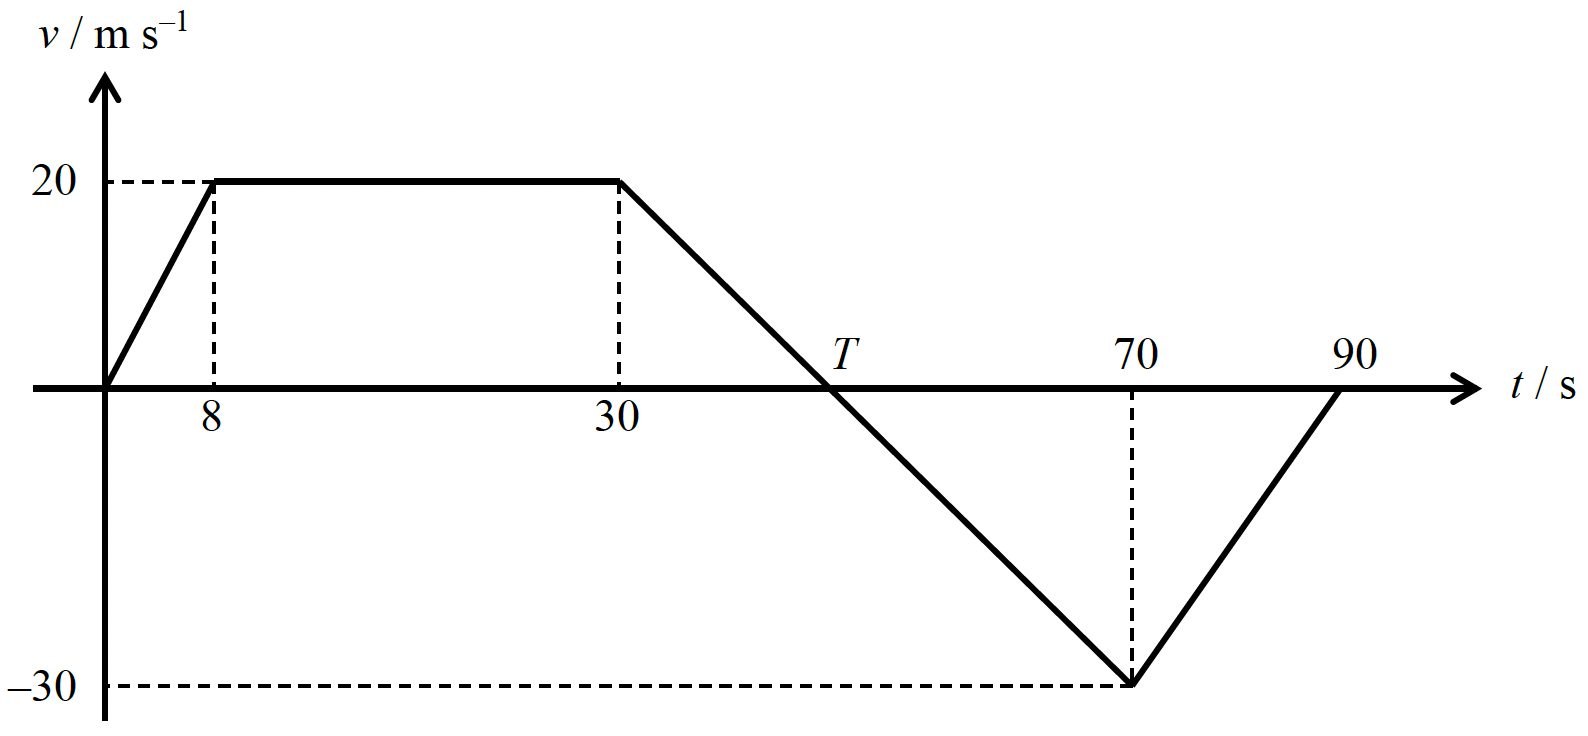
\includegraphics[width=\textwidth]{../../assets/c30be131.png}
    \end{figure}
\end{frame}
\begin{frame}[t]{例題}
    \begin{itemize}
        \item [(a)] 求 T 的值。
    \end{itemize}
\end{frame}
\begin{frame}[t]{例題}
    \begin{itemize}
        \item [(b)] 求車在時間 $t = 0-90$ s 期間所行走的距離和位移量值。
    \end{itemize}
\end{frame}

\begin{frame}{運動方程 Equations of motions}
    當一個物件沿直線作勻加速運動,設它的位移、初速度、末速度、加速度和時間分別是 $\mathit{s}$、$\mathit{u}$、$\mathit{v}$、$\mathit{a}$ 和 $\mathit{t}$,則有以下描述勻加速運動的方程︰
    \begin{figure}[h!]
        \centering
        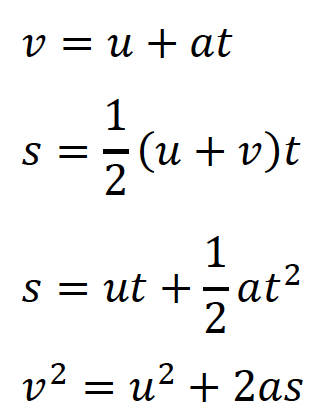
\includegraphics[width=.2\textwidth]{../../assets/6d3f21f0.png}
    \end{figure}
\end{frame}

\begin{frame}[t]{例題}
    一隻狗沿直線以 \acc{6.3} 加速,求牠從靜止加速 3 s 後的速度和位移。
\end{frame}
\begin{frame}[t]{例題}
    一艘船沿直線從 \kmh{60} 勻加速至 \kmh{100},過程中航行 30 m。求快艇加速度和加速需時。
\end{frame}
\begin{frame}[t]{例題}
    汽車在交通意外中緊急剎車,留下長 20 m 的剎車痕。調査人員發現,相同的汽車以 \kmh{50} 行駛時緊急剎車,會留下長 10 m 的剎車痕。假設上述兩輛汽車以相同的恆減速度剎車。試估算發生意外的汽車在剎車前一刻的速率。
\end{frame}
\begin{frame}[t]{例題}
    汽車沿直路以 \kmh{60} 行駛,司機看見前方 30 m 有障礙物,於是剎停汽車。司機的反應時間是 0.9 s。剎車時,汽車以 \acc{7} 均勻地減慢。根據上述資料,求 (a) 反應距離、(b) 制動距離;及 (c) 停車距離。 由此,解釋汽車會否撞上障礙物。
\end{frame}


\end{document}